
        \documentclass[addpoints,spanish, 12pt,a4paper]{exam}
        %\documentclass[answers, spanish, 12pt,a4paper]{exam}
        
        \printanswers
        \pointpoints{punto}{puntos}
        \hpword{Puntos:}
        \vpword{Puntos:}
        \htword{Total}
        \vtword{Total}
        \hsword{Resultado:}
        \hqword{Ejercicio:}
        \vqword{Ejercicio:}

        \usepackage[utf8]{inputenc}
        \usepackage[spanish]{babel}
        \usepackage{eurosym}
        %\usepackage[spanish,es-lcroman, es-tabla, es-noshorthands]{babel}


        \usepackage[margin=1in]{geometry}
        \usepackage{amsmath,amssymb}
        \usepackage{multicol, xparse}

        \usepackage{yhmath}

        \usepackage{verbatim}
        %\usepackage{pstricks}


        \usepackage{graphicx}
        \graphicspath{{../img/}}




        \let\multicolmulticols\multicols
        \let\endmulticolmulticols\endmulticols
        \RenewDocumentEnvironment{multicols}{mO{}}
         {%
          \ifnum#1=1
            #2%
          \else % More than 1 column
            \multicolmulticols{#1}[#2]
          \fi
         }
         {%
          \ifnum#1=1
          \else % More than 1 column
            \endmulticolmulticols
          \fi
         }
        \renewcommand{\solutiontitle}{\noindent\textbf{Sol:}\enspace}

        \newcommand{\samedir}{\mathbin{\!/\mkern-5mu/\!}}

        \newcommand{\class}{1º Bachillerato}
        \newcommand{\examdate}{\today}

        %\newcommand{\tipo}{A}


        \newcommand{\timelimit}{80 minutos}

        \renewcommand{\solutiontitle}{\noindent\textbf{Solución:}\enspace}


        \pagestyle{head}
        \firstpageheader{
\includegraphics[width=0.2\columnwidth]{header_left}}{\textbf{Departamento de Matemáticas\linebreak \class}\linebreak \examnum}{
\includegraphics[width=0.1\columnwidth]{header_right}}
        \runningheader{\class}{\examnum}{Página \thepage\ of \numpages}
        \runningheadrule
        
        \pointsinrightmargin % Para poner las puntuaciones a la derecha. Se puede cambiar. Si se comenta, sale a la izquierda.
        \extrawidth{-2.4cm} %Un poquito más de margen por si ponemos textos largos.
        \marginpointname{ \emph{\points}}

        
            \newcommand{\tipo}{A}\newcommand{\examnum}{Final 3ª evaluación}
        \begin{document}
        \noindent
        \begin{tabular*}{\textwidth}{l @{\extracolsep{\fill}} r @{\extracolsep{6pt}} }
        \textbf{Nombre:} \makebox[3.5in]{\hrulefill} & \textbf{Fecha:}\makebox[1in]{\hrulefill} \\
         & \\
        \textbf{Tiempo: \timelimit} & Tipo: \tipo 
        \end{tabular*}
        \rule[2ex]{\textwidth}{2pt}
        Esta prueba tiene \numquestions\ ejercicios. La puntuación máxima es de \numpoints. 
        La nota final de la prueba será la parte proporcional de la puntuación obtenida sobre la puntuación máxima. 

        \begin{center}


        \addpoints
             %\gradetable[h][questions]
            \pointtable[h][questions]
        \end{center}

        \noindent
        \rule[2ex]{\textwidth}{2pt}

        \begin{questions}

%        \question Calcula los siguientes límites:
%        \begin{multicols}{1}
%        \begin{parts} \part[1] $$\lim_{x \to 3}\left(\frac{3 x^{2} - 11 x + 6}{x^{3} - 3 x^{2} + x - 3}\right)$$  \begin{solution}   $\frac{7}{10}$   \end{solution} \part[1] $$\lim_{x \to \infty} e^{1 - x}$$  \begin{solution}   $0$   \end{solution} \part[1] $$\lim_{x \to -2}\left(\frac{x^{3} + x^{2} - x + 2}{x^{2} + 4 x + 4}\right)$$  \begin{solution}   No existe el límite   \end{solution} \part[2] $$\lim_{x \to 2} \left(\frac{x^{3} - 4}{x^{2}}\right)^{\frac{1}{x - 2}}$$  \begin{solution}   $e^{2}$   \end{solution}
%        \end{parts}
%        \end{multicols}
        
        \question Las notas de 4 alumnos en las asignaturas $X$ e $Y$ han sido:
        
\begin{tabular}{l|cccc}
{} &  Ana & Juan  &  Pepe &   Luisa \\
\hline
X &  5 &  8 &  3 &  10 \\
Y &  6 &  9 &  2 &  10 \\
\hline
\end{tabular}
\begin{solution}
        \begin{tabular}{lrrrrr}
\hline
        &    x &     y &   $x\cdot y$ &   $x^2$ &   $y^2$ \\
\hline
 0      &  5   &  6    &           30 &    25   &   36    \\
 1      &  8   &  9    &           72 &    64   &   81    \\
 2      &  3   &  2    &            6 &     9   &    4    \\
 3      & 10   & 10    &          100 &   100   &  100    \\
 Sumas  & 26   & 27    &          208 &   198   &  221    \\
 Medias &  6.5 &  6.75 &           52 &    49.5 &   55.25 \\
\hline
\end{tabular}
\\ \\ Las medias son: \\$\overline{x}=\frac{\Sigma{x_i}}{N}=\frac{26.0}{4}=6.5$. $\overline{y}=\frac{\Sigma{y_i}}{N}=\frac{27.0}{4}=6.75$.  El centro de gravedad es: $(6.5,6.75)$ \\ \\ Varianzas y covarianzas\\ $\sigma_x=\sqrt{\frac{\sum{x_i^2}}{N}-\overline{x}^2}=\sqrt{\frac{198.0}{4}-6.5^2}=2.69258240356725$.\\ $\sigma_y=\sqrt{\frac{\sum{y_i^2}}{N}-\overline{y}^2}=\sqrt{\frac{221.0}{4}-6.75^2}=3.11247489949718$.\\ $\sigma_{xy}=\frac{\sum{x_i \cdot y_i}}{N}-\overline{x}\cdot \overline{y}=\frac{208.0}{4}-6.5\cdot 6.75=8.125$. \\ \\ Correlación\\ $r=\dfrac{\sigma_{xy}}{\sigma_x \cdot \sigma_y}=\frac{8.125}{2.69258240356725\cdot 3.11247489949718}=0.969501551920812$. \\ \\ Recta de regresión: \\ La pendiente es: 1.12068965517241, la ordenada en el origen: -0.534482758620689, El coeficiente de correlación:0.969501551920812 y la recta de regresión: $y = 1.12068965517241 x - 0.534482758620689$.
$y(7)=7.31034482758618$
\end{solution}

\begin{parts}
    \part[1] Calcula las medias y desviaciones típicas de las asignaturas $X$ e $Y$
    \part[1] Obtén la recta de regresión de Y sobre X y estima con ella la nota correspondiente a la asignatura $Y$ de in alumno que ha sacado un 7 en la asignatura $X$.
\end{parts}


% \question Luis es saltador de altura, y en el 70\% de sus saltos consigue superar los 2.10 m. Sabiendo que en una competición tiene que saltar tres veces, halla la probabilidad de que:

% \begin{parts} 
% \part[1]  En todas supere los 2.10 m.  \begin{solution}  $ 0.3430$  \end{solution} 
% \part[1]  No los supere en ninguna  \begin{solution}  $0.02700 $  \end{solution}
% \part[1]  Si su primer salto fue nulo, supere los 2.10 m en, al menos, una ocasión.  \begin{solution}  $0.9100$  \end{solution}
%         \end{parts}

\question En una urna hay 10 bolas blancas y 3 negras. Se extrae una bola al azar y, sin verla ni
reemplazarla, se extrae una segunda bola.
\begin{parts}
    \part[1] ¿Cuál es la probabilidad de que la segunda bola extraída sea negra?\begin{solution}$\frac{3}{13}$\end{solution}
    
    \part[1] Sabiendo que la segunda bola ha sido negra, calcule la probabilidad de que la primera bola extraída fuera negra también.\begin{solution}$\frac{1}{6}$\end{solution}
\end{parts}

\question Un examen de tipo test consta de 8 preguntas, cada una con cinco respuestas, de las cuales solo
una es correcta. Si un alumno contesta al azar:
\begin{parts}
    \part[1] ¿Cuál es la probabilidad de que conteste correctamente 4 preguntas?\begin{solution}$0.0458752000000000$\end{solution}
    \part[1] ¿Y la de que conteste bien 2 preguntas o más?\begin{solution}$0.496683520000000$\end{solution}

\end{parts}
        
\question Una máquina produce recipientes cuyas capacidades siguen una distribución normal de media 100 cl y de desviación típica 0,9.
\begin{parts}
    \part[1] Calcula la probabilidad de que la capacidad de un recipiente elegido al azar sea menor que 101 \begin{solution}$0.866739737097495$\end{solution}
    \part[1] Calcula la probabilidad de que la capacidad de un recipiente elegido al azar sea mayor que 99\begin{solution}$0.866739737097495$\end{solution}
    \part[1] Si el fabricante considera que un recipiente es defectuoso si su capacidad no está entre 99 y 101. ¿Qué
probabilidad tiene un recipiente de ser considerado defectuoso?\begin{solution}$1-0.733479474194989=0.266520525805011$\end{solution}
\end{parts}

        % \question Determina el dominio de definición de las siguientes funciones:
        % \begin{parts}
        % % reduce_inequalities([(x**2-x)/(x+2)>=0]).as_set()
        % \part[1] $f(x)=\sqrt{\dfrac{x^2 -x}{x+2}}$\begin{solution}  $\left(-2, 0\right] \cup \left[1, \infty\right)$\end{solution}
        % \part[1] $f(x)=\dfrac{3x+2}{x^4-5x^2-36}$\begin{solution}$\left(-\infty, -3\right] \cup \left[3, \infty\right)$\end{solution}
        % \end{parts}
        
        \question Dada la función $f(x)=\dfrac{3 x - 2}{2}$:
                \begin{parts} \part[1] Calcula $f^{-1}(x)$, es decir la inversa de $f(x)$  \begin{solution}   $f^{-1}(x)=\frac{2 x}{3} + \frac{2}{3}$ \\ $f^{-1} \circ f(x)=x=x$ \\ 
               \end{solution}
               \part[1] Comprueba que efectivamente son inversas
        % \part[1] $f(x)=\frac{x}{- x + 1}$  \begin{solution}   $f^{-1}(x)=\frac{x}{x + 1}$ \\ $f^{-1} \circ f(x)=\frac{x}{\left(- x + 1\right) \left(\frac{x}{- x + 1} + 1\right)}=x$   \end{solution}
        \end{parts}
        
        
        \question Calcula los siguientes límites:
        \begin{multicols}{1}
        \begin{parts} 
        \part[1] $$\lim_{x \to -1}\left(x^{2} - 3\right)$$  \begin{solution}   $\lim_{x \to -1^-}\left(x^{2} - 3\right)=-2$ y  \\ $\lim_{x \to -1^+}\left(x^{2} - 3\right)=-2$   \end{solution} 
        \part[1] $$\lim_{x \to 2}\left(\frac{x^{3} - 2 x^{2} + 2 x - 4}{3 x^{2} - 8 x + 4}\right)$$  \begin{solution}   $\frac{3}{2}$   \end{solution} 
        % \part[1] $$\lim_{x \to -\infty} e^{x - 1}$$  \begin{solution}   $0$   \end{solution} 
        % \part[1] $$\lim_{x \to -1}\left(\frac{x^{3} + 1}{x^{2} + 2 x + 1}\right)$$  \begin{solution}   No existe el límite   \end{solution} 
        % \part[2] $$\lim_{x \to 3} \left(\frac{x^{2} - x}{x + 3}\right)^{\frac{1}{x - 3}}$$  \begin{solution}   $e^{\frac{2}{3}}$   \end{solution}
        \part[2] $$\lim_{x \to \infty}\left(\dfrac{x^{2} - 1}{x} - \dfrac{2 x^{2} + 1}{2 x - 1}\right)$$\begin{solution}$-\frac{1}{2}$\end{solution}
        
        \end{parts}
        \end{multicols}
        
        
        
%        \question Dada la función:$f(x)=\frac{x^{2} - 2 x + 1}{2 x + 3}$, calcular:
%        \begin{multicols}{1}
%        \begin{parts} \part[1] Dominio de $f(x)$  \begin{solution}   $Dom(f)=\left(-\infty, - \frac{3}{2}\right) \cup \left(- \frac{3}{2}, \infty\right)$\\ \resizebox{0.4\textwidth}{!}{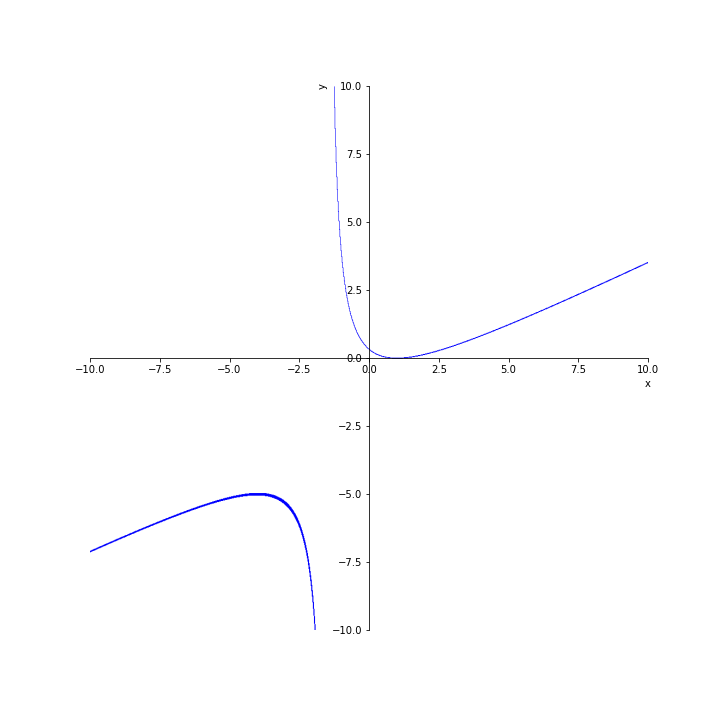
\includegraphics[width=1\columnwidth]{fin301-0}}   \end{solution} \part[2] Asíntotas verticales, horizontales y oblicuas, en caso que existan  \begin{solution}   Asíntotas:\\A.V. $x=-3/2$\\A.O. $y=\frac{x}{2} - \frac{7}{4}$ \\A.O. $y=\frac{x}{2} - \frac{7}{4}$ \\   \end{solution}
%        \end{parts}
%        \end{multicols}
%        \question Dada la función:$f(x)=\frac{- x^{2} - x + 3}{x^{2} + x - 2}$, calcular:
%        \begin{multicols}{1}
%        \begin{parts} \part[1] Dominio de $f(x)$  \begin{solution}   $Dom(f)=\left(-\infty, -2\right) \cup \left(-2, 1\right) \cup \left(1, \infty\right)$\\ \resizebox{0.4\textwidth}{!}{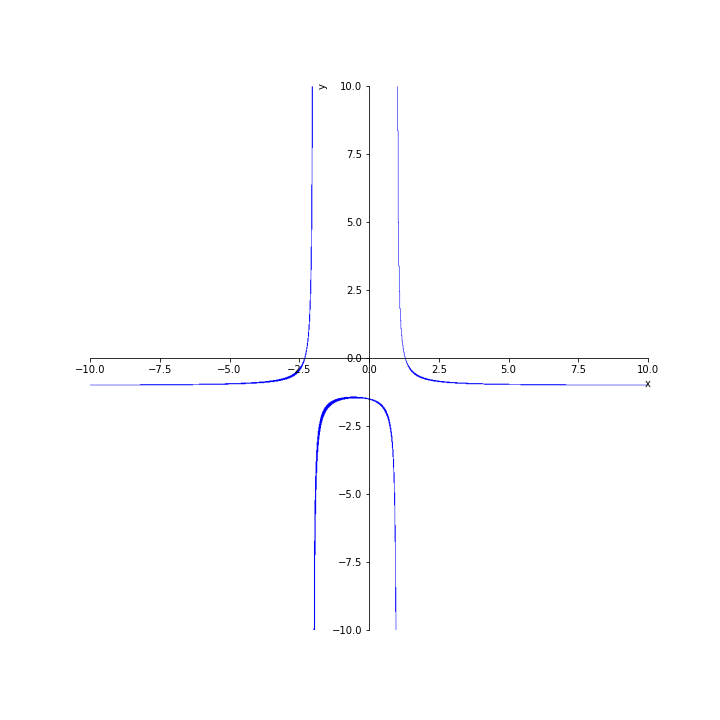
\includegraphics[width=1\columnwidth]{fin301-1}}   \end{solution} \part[2] Asíntotas verticales, horizontales y oblicuas, en caso que existan  \begin{solution}   Asíntotas:\\A.V. $x=-2$\\, A.V. $x=1$\\A.H. $y=-1$\\A.H. $y=-1$\\A.O. $y=-1$ \\A.O. $y=-1$ \\   \end{solution}
%        \end{parts}
%        \end{multicols}


        % \question Dada la función:$f(x)=\sqrt{\frac{x}{x - 1}}$, calcular:
        % \begin{multicols}{1}
        % \begin{parts} \part[1] Dominio de $f(x)$  \begin{solution}   $Dom(f)=\left(-\infty, 0\right] \cup \left(1, \infty\right)$\\ \resizebox{0.4\textwidth}{!}{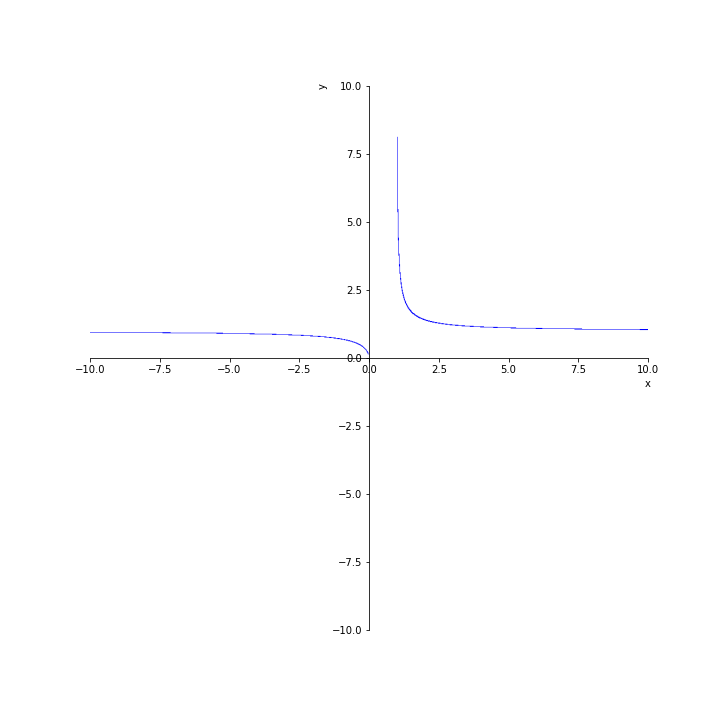
\includegraphics[width=1\columnwidth]{fin301-2}}   \end{solution} \part[2] Asíntotas verticales, horizontales y oblicuas, en caso que existan  \begin{solution}   Asíntotas:\\A.V. $x=1$\\A.H. $y=1$\\A.H. $y=1$\\A.O. $y=1$ \\A.O. $y=1$ \\   \end{solution}
        % \end{parts}
        % \end{multicols}


%        \question Estudia en qué puntos de $\mathbb{R}$ la función no es continua: 
%        \begin{multicols}{1}
%        \begin{parts} \part[2] $f(x)=\begin{cases} \frac{2 x^{2} + 7 x + 3}{x^{2} - 9} & \text{si}\: x \leq -2 \\\frac{\sqrt{x + 3} - 1}{x^{2} + 2 x} & \text{si} \: x > -2\end{cases}$  \begin{solution}   Singularidades de las expresiones analíticas: $\left\{-3, 0\right\}$.\\ Posibles discontinuidades en los extremos de los trozos:-2.\\En -2 no es continua porque no existe límite. Límites laterales: $\frac{3}{5}$ y $- \frac{1}{4}$   \end{solution}
%        \end{parts}
%        \end{multicols}
        
        
        % \question Estudia en qué puntos de $\mathbb{R}$ la función no es continua: 
        % \begin{multicols}{1}
        % \begin{parts} \part[2] $f(x)=\begin{cases} \frac{x^{2} - 4}{x^{2} - 3 x + 2} & \text{si}\: x < 2 \\4 & \text{si}\: 2\leq x < 5 \\e^{x - 5} + 3 & \text{si}\: x > 5 \end{cases}$  \begin{solution}   Singularidades de las expresiones analíticas: $\left\{1\right\}$.\\ Posibles discontinuidades en los extremos de los trozos:2, 5.\\En 2 es continua ya que hay límite y $\lim = f(2)=4$. \\En 5 es continua ya que hay límite y $\lim = f(5)=4$   \end{solution}
        % \end{parts}
        % \end{multicols}
        
%        \question Halla a y b de modo que las siguientes funciones sean continuas:
%        \begin{multicols}{1}
%        \begin{parts} \part[2] $$f(x)=\begin{cases} a + e^{x + 2} & \text{si}\: x \leq -2 \\\frac{x + 1}{3 - x} & \text{si}\: -2 < x < 1 \\b x + 3 & \text{si}\: x \geq 1 \end{cases}$$  \begin{solution}   $\left\{ a : - \frac{6}{5}, \  b : -2\right\}$   \end{solution}
%        \end{parts}
%        \end{multicols}
        
        % \question Halla a y b de modo que las siguientes funciones sean continuas:
        % \begin{multicols}{1}
        % \begin{parts} \part[2] $$f(x)=\begin{cases} a + e^{x + 3} & \text{si}\: x \leq -3 \\\frac{x + 2}{4 - x} & \text{si}\: -3 < x < 1 \\b x + 6 & \text{si}\: x \geq 1 \end{cases}$$  \begin{solution}   $\left\{ a : - \frac{8}{7}, \  b : -5\right\}$   \end{solution}
        % \end{parts}
        % \end{multicols}
        
        
        
%        \question Deriva las siguientes funciones (simplificando el resultado al máximo):
%        \begin{multicols}{1}
%        \begin{parts} \part[1] $y=\frac{3 x^{2} - 2 x + 1}{\left(x - 1\right)^{2}}$  \begin{solution}   $y'=- \frac{4 x}{x^{3} - 3 x^{2} + 3 x - 1}$   \end{solution} \part[1] $y=\sqrt{\sqrt{x} + 1}$  \begin{solution}   $y'=\frac{1}{4 \sqrt{x} \sqrt{\sqrt{x} + 1}}$   \end{solution} \part[1] $y=\frac{\log{\left(x^{2} \right)}}{x}$  \begin{solution}   $y'=\frac{2 - \log{\left(x^{2} \right)}}{x^{2}}$   \end{solution} \part[1] $y=3 \sin{\left(\cos{\left(2 x \right)} \right)}$  \begin{solution}   $y'=- 6 \sin{\left(2 x \right)} \cos{\left(\cos{\left(2 x \right)} \right)}$   \end{solution}
%        \end{parts}
%        \end{multicols}
        
        % \question Deriva las siguientes funciones (simplificando el resultado al máximo):
        % \begin{multicols}{1}
        % \begin{parts} \part[1] $y=\frac{2 x^{2} - 2 x + 1}{\left(x - 1\right)^{2}}$  \begin{solution}   $y'=- \frac{2 x}{x^{3} - 3 x^{2} + 3 x - 1}$   \end{solution} \part[1] $y=\sqrt{2 - \sqrt{x}}$  \begin{solution}   $y'=- \frac{1}{4 \sqrt{x} \sqrt{2 - \sqrt{x}}}$   \end{solution} \part[1] $y=\frac{\log{\left(x \right)}}{x}$  \begin{solution}   $y'=\frac{1 - \log{\left(x \right)}}{x^{2}}$   \end{solution} \part[1] $y=2 \cos{\left(\sin{\left(2 x \right)} \right)}$  \begin{solution}   $y'=- 4 \sin{\left(\sin{\left(2 x \right)} \right)} \cos{\left(2 x \right)}$   \end{solution}
        % \end{parts}
        % \end{multicols}
        
%        \question Se dispone de dos cajas, la caja A contiene 3 bolas moradas y 2 bolas rojas; mientras que la caja B contiene 4
%    bolas moradas y 4 rojas.
%        \begin{multicols}{1}
%        \begin{parts} \part[2] Se escoge una bola cualquiera de la caja A y se pasa a la caja B. Posteriormente se saca una
%    bola de la caja B. ¿Cuál es la probabilidad de que la bola extraída de la caja B sea morada?.   \begin{solution}   $\frac{3}{5}\cdot\frac{5}{9}+\frac{2}{5}\cdot\frac{4}{9}=\frac{23}{45}$   \end{solution} \part[2] Ahora volvemos a la situación original de las cajas. Seleccionamos una caja al azar y se saca una bola 
%    que resulta ser roja. ¿Cuál es la probabilidad de que esa
%    bola sea de la caja A?  \begin{solution}   $\dfrac{\frac{1}{2}\cdot\frac{2}{5}}{\frac{1}{2}\cdot\frac{2}{5}+\frac{1}{2}\cdot\frac{1}{2}}=\frac{4}{9}$   \end{solution}
%        \end{parts}
%        \end{multicols}

    %     \question Se dispone de dos cajas, la caja A contiene 3 bolas verdes y 2 bolas blancas; mientras que la caja B contiene 4
    % bolas verdes y 4 blancas.
    %     \begin{multicols}{1}
    %     \begin{parts} \part[2] Se escoge una bola cualquiera de la caja A y se pasa a la caja B. Posteriormente se saca una
    % bola de la caja B. ¿Cuál es la probabilidad de que la bola extraída de la caja B sea verde?.   \begin{solution}   $\frac{3}{4}\cdot\frac{5}{9}+\frac{1}{4}\cdot\frac{4}{9}=\frac{19}{36}$   \end{solution} \part[2] Ahora volvemos a la situación original de las cajas. Seleccionamos una caja al azar y se saca una bola 
    % que resulta ser blanca. ¿Cuál es la probabilidad de que esa
    % bola sea de la caja A?  \begin{solution}   $\dfrac{\frac{1}{2}\cdot\frac{1}{4}}{\frac{1}{2}\cdot\frac{1}{4}+\frac{1}{2}\cdot\frac{1}{2}}=\frac{1}{3}$   \end{solution}
    %     \end{parts}
    %     \end{multicols}

        
    \end{questions}
    
    \newgeometry{left=1 cm,bottom=2cm}
% \begin{landscape}
\begin{table}
% \Large
\centering

% \caption{Extracto de tabla de probabilidades de la \textbf{normal estándar $Z(0,1)$}}
\caption{Tabla de probabilidades de la \textbf{normal estándar $Z(0,1)$}}
\label{my-label}

\begin{tabular}{l|llllllllll}
z   & 0       & 0,01    & 0,02    & 0,03    & 0,04    & 0,05    & 0,06    & 0,07    & 0,08    & 0,09    \\
\hline
0   & 0,5     & 0,50399 & 0,50798 & 0,51197 & 0,51595 & 0,51994 & 0,52392 & 0,5279  & 0,53188 & 0,53586 \\
0,1 & 0,53983 & 0,5438  & 0,54776 & 0,55172 & 0,55567 & 0,55962 & 0,56356 & 0,56749 & 0,57142 & 0,57535 \\
0,2 & 0,57926 & 0,58317 & 0,58706 & 0,59095 & 0,59483 & 0,59871 & 0,60257 & 0,60642 & 0,61026 & 0,61409 \\
0,3 & 0,61791 & 0,62172 & 0,62552 & 0,6293  & 0,63307 & 0,63683 & 0,64058 & 0,64431 & 0,64803 & 0,65173 \\
0,4 & 0,65542 & 0,6591  & 0,66276 & 0,6664  & 0,67003 & 0,67364 & 0,67724 & 0,68082 & 0,68439 & 0,68793 \\
0,5 & 0,69146 & 0,69497 & 0,69847 & 0,70194 & 0,7054  & 0,70884 & 0,71226 & 0,71566 & 0,71904 & 0,7224  \\
0,6 & 0,72575 & 0,72907 & 0,73237 & 0,73565 & 0,73891 & 0,74215 & 0,74537 & 0,74857 & 0,75175 & 0,7549  \\
0,7 & 0,75804 & 0,76115 & 0,76424 & 0,7673  & 0,77035 & 0,77337 & 0,77637 & 0,77935 & 0,7823  & 0,78524 \\
0,8 & 0,78814 & 0,79103 & 0,79389 & 0,79673 & 0,79955 & 0,80234 & 0,80511 & 0,80785 & 0,81057 & 0,81327 \\
0,9 & 0,81594 & 0,81859 & 0,82121 & 0,82381 & 0,82639 & 0,82894 & 0,83147 & 0,83398 & 0,83646 & 0,83891 \\
1   & 0,84134 & 0,84375 & 0,84614 & 0,84849 & 0,85083 & 0,85314 & 0,85543 & 0,85769 & 0,85993 & 0,86214 \\
1,1 & 0,86433 & 0,8665  & 0,86864 & 0,87076 & 0,87286 & 0,87493 & 0,87698 & 0,879   & 0,881   & 0,88298 \\
1,2 & 0,88493 & 0,88686 & 0,88877 & 0,89065 & 0,89251 & 0,89435 & 0,89617 & 0,89796 & 0,89973 & 0,90147 \\
1,3 & 0,9032  & 0,9049  & 0,90658 & 0,90824 & 0,90988 & 0,91149 & 0,91309 & 0,91466 & 0,91621 & 0,91774 \\
1,4 & 0,91924 & 0,92073 & 0,9222  & 0,92364 & 0,92507 & 0,92647 & 0,92785 & 0,92922 & 0,93056 & 0,93189 \\
1,5 & 0,93319 & 0,93448 & 0,93574 & 0,93699 & 0,93822 & 0,93943 & 0,94062 & 0,94179 & 0,94295 & 0,94408 \\
1,6 & 0,9452  & 0,9463  & 0,94738 & 0,94845 & 0,9495  & 0,95053 & 0,95154 & 0,95254 & 0,95352 & 0,95449 \\
1,7 & 0,95543 & 0,95637 & 0,95728 & 0,95818 & 0,95907 & 0,95994 & 0,9608  & 0,96164 & 0,96246 & 0,96327 \\
1,8 & 0,96407 & 0,96485 & 0,96562 & 0,96638 & 0,96712 & 0,96784 & 0,96856 & 0,96926 & 0,96995 & 0,97062 \\
1,9 & 0,97128 & 0,97193 & 0,97257 & 0,9732  & 0,97381 & 0,97441 & 0,975   & 0,97558 & 0,97615 & 0,9767  \\
2   & 0,97725 & 0,97778 & 0,97831 & 0,97882 & 0,97932 & 0,97982 & 0,9803  & 0,98077 & 0,98124 & 0,98169 \\
2,1 & 0,98214 & 0,98257 & 0,983   & 0,98341 & 0,98382 & 0,98422 & 0,98461 & 0,985   & 0,98537 & 0,98574 \\
2,2 & 0,9861  & 0,98645 & 0,98679 & 0,98713 & 0,98745 & 0,98778 & 0,98809 & 0,9884  & 0,9887  & 0,98899 \\
2,3 & 0,98928 & 0,98956 & 0,98983 & 0,9901  & 0,99036 & 0,99061 & 0,99086 & 0,99111 & 0,99134 & 0,99158 \\
2,4 & 0,9918  & 0,99202 & 0,99224 & 0,99245 & 0,99266 & 0,99286 & 0,99305 & 0,99324 & 0,99343 & 0,99361 \\
2,5 & 0,99379 & 0,99396 & 0,99413 & 0,9943  & 0,99446 & 0,99461 & 0,99477 & 0,99492 & 0,99506 & 0,9952  \\
2,6 & 0,99534 & 0,99547 & 0,9956  & 0,99573 & 0,99585 & 0,99598 & 0,99609 & 0,99621 & 0,99632 & 0,99643 \\
2,7 & 0,99653 & 0,99664 & 0,99674 & 0,99683 & 0,99693 & 0,99702 & 0,99711 & 0,9972  & 0,99728 & 0,99736 \\
2,8 & 0,99744 & 0,99752 & 0,9976  & 0,99767 & 0,99774 & 0,99781 & 0,99788 & 0,99795 & 0,99801 & 0,99807 \\
2,9 & 0,99813 & 0,99819 & 0,99825 & 0,99831 & 0,99836 & 0,99841 & 0,99846 & 0,99851 & 0,99856 & 0,99861 \\
3   & 0,99865 & 0,99869 & 0,99874 & 0,99878 & 0,99882 & 0,99886 & 0,99889 & 0,99893 & 0,99896 & 0,999   \\
3,1 & 0,99903 & 0,99906 & 0,9991  & 0,99913 & 0,99916 & 0,99918 & 0,99921 & 0,99924 & 0,99926 & 0,99929 \\
3,2 & 0,99931 & 0,99934 & 0,99936 & 0,99938 & 0,9994  & 0,99942 & 0,99944 & 0,99946 & 0,99948 & 0,9995  \\
3,3 & 0,99952 & 0,99953 & 0,99955 & 0,99957 & 0,99958 & 0,9996  & 0,99961 & 0,99962 & 0,99964 & 0,99965 \\
3,4 & 0,99966 & 0,99968 & 0,99969 & 0,9997  & 0,99971 & 0,99972 & 0,99973 & 0,99974 & 0,99975 & 0,99976 \\
3,5 & 0,99977 & 0,99978 & 0,99978 & 0,99979 & 0,9998  & 0,99981 & 0,99981 & 0,99982 & 0,99983 & 0,99983 \\
3,6 & 0,99984 & 0,99985 & 0,99985 & 0,99986 & 0,99986 & 0,99987 & 0,99987 & 0,99988 & 0,99988 & 0,99989 \\
3,7 & 0,99989 & 0,9999  & 0,9999  & 0,9999  & 0,99991 & 0,99991 & 0,99992 & 0,99992 & 0,99992 & 0,99992 \\
3,8 & 0,99993 & 0,99993 & 0,99993 & 0,99994 & 0,99994 & 0,99994 & 0,99994 & 0,99995 & 0,99995 & 0,99995 \\
3,9 & 0,99995 & 0,99995 & 0,99996 & 0,99996 & 0,99996 & 0,99996 & 0,99996 & 0,99996 & 0,99997 & 0,99997 \\
4   & 0,99997 & 0,99997 & 0,99997 & 0,99997 & 0,99997 & 0,99997 & 0,99998 & 0,99998 & 0,99998 & 0,99998
\end{tabular}
\end{table}
% \end{landscape}
\restoregeometry
    \end{document}
    